\documentclass{article}
\usepackage{amsmath, amssymb, amsthm}
\usepackage{graphicx} % For adding images
\graphicspath{{images/}}

% Customization
\newtheorem{definition}{Definition}
\theoremstyle{definition}
\newtheorem{example}{Example}[section]
%GEOMETRY
\usepackage[letterpaper, top=1.0in, bottom=1.0in, left=1.0in, right=1.0in, heightrounded]{geometry}

%line height
\renewcommand{\baselinestretch}{1.15}

%parskip and parindent
\setlength{\parindent}{0pt}
\setlength{\parskip}{0.8em}

\begin{document}
%TODO: add title page and tables of contents

\section{Chapter 1}

\subsection*{1.0}

There are 6 main issues we will focus on in economics:
\begin{itemize}
    \item \begin{definition}Productivity Growth\end{definition}
    Productivity is measured by ${Productivity=Output/Worker}$\\
    Incentives lead to productivity growth.
    \item \begin{definition} Population Growth\end{definition}
    Canada is open to immigrants, we have a low birth rate compared to past generations.
    No population growth leads to less workers, meaning workers must work harder.
    There are benefits and costs of having children.
    \item \begin{definition}Climate Change\end{definition}
    Cities in Canada and moving towards bodies of waters. Risk of submersion.
    Need to think about city design and allocation of people and resources.
    \begin{example}
        Farmers' harvests are affected by climate change. Impacts their income.
    \end{example}
    Economic impact of climate change is a big issue.
    \item \begin{definition}Technological Change\end{definition}
    Changing many industries, including education.
    Automation, job losses but also new job markets.
    Presently, might technological change may seem to be bad news but the future brings changes.
    \item \begin{definition}Protectionism\end{definition}
    Has been, unfortunately, on the rise over 20-40 years.
    Opposed to trade or comes with conditions.
    Countries have decided to tie trades to labour and climate conditions and standards.
    Free trade resists protectionism.
    \item \begin{definition}Inequality\end{definition}
    Highly undesirable, unless you are at the top of the distribution.
    Not within your control.
    Income inequality is problematic but has a deeper understanding. There is a difference between unfair and inequal.
    Need to analyze individual potential.
\end{itemize}

\subsection{}
\begin{definition}
    Economics is a social science that studies how we allocate limited resources
    to satisfy unlimited wants.
\end{definition}
\begin{definition}
    Social science is the study of people.
\end{definition}
Is the allocation of resources fair? just? efficient?
By resources we mean:
\begin{itemize}
    \item Land (T)
    \item Labour (L)
    \item Capital (K) 
\end{itemize}
Note: Money is not a resource, it is a means of making exchange easier.
With Land, Labour or Capital you could make use of them on a island alone.

These resources are limited or scarce but \textbf{our wants are unlimited}. Even billionaires give away their money for their wants.
Scarcity $\rightarrow$ Choice.
\begin{figure}[h!]
    \begin{minipage}{\textwidth}
        \centering
        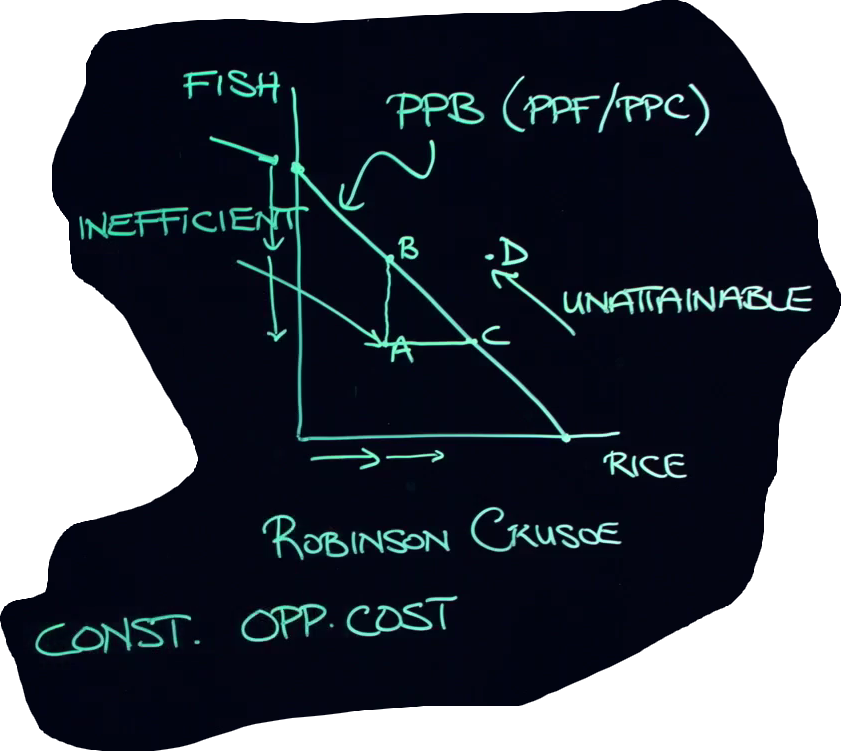
\includegraphics[width=0.5\textwidth]{RobinsonConstant.png}
        \caption[Constant Opportunity Cost]{Robinson Crusoe\footnote[1]{Story of a life of comfort to a solitary existence on a deserted island}'s Constant Opportunity Cost}
    \end{minipage}
\end{figure}
\begin{center}
\end{center}
Naturally we try to equalize the values of rice and fish (EQUITY).
If we used all of Crusoe's resources we would get a linear line (PPB/PPF/PPC meaning Production Possibility). Say that point A is below the line. This means it is potential with his resources but we say it is \textbf{inefficient}.
Same with point B and C but they maximize his resources. Point D is above the line and is \textbf{unattainable}, meaning he cannot achieve it.

\begin{definition}
    Opportunity Cost is the value of the next best alternative forgone.
    \begin{example}
    If Crusoe has maximized his use of resources, to acquire more rice, Crusoe must give up some fish.
    The cost is constant in this example.
    \end{example}
    Note: In real life, a constant opportunity cost is generally not realistic.
\end{definition}
Imagine Crusoe's opportunity cost is no longer constant but increasing.
The graph of his resources would be a slope.\\
\begin{figure}[h!]
    \centering
    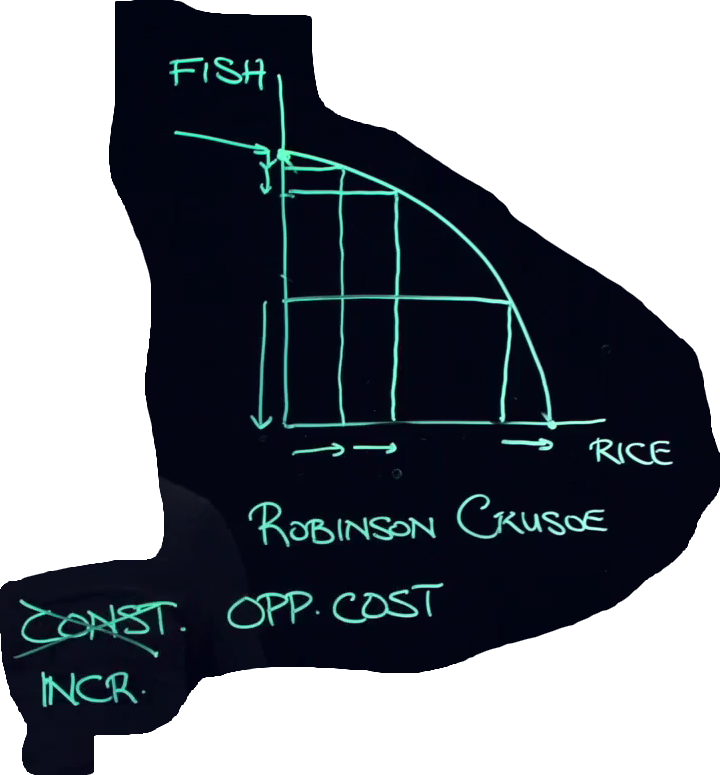
\includegraphics[width=0.5\textwidth]{RobinsonIncreasing.png}
    \caption{Robinson Crusoe's Increasing Opportunity Cost}
\end{figure}
Crusoe is able to give up the inefficent methods of obtaining fish/rice for the other initially.
To obtain more and more of the other, he must give up more and more of the other. This is the law of increasing opportunity cost.

\subsection{}

\begin{definition}
    Market Economy is an economy where resources are allocated through the decentralized decisions of many firms and households as they interact in markets for goods and services.
    The economy is characterized by being self-organizing and efficient.
    We assume that the agents of the market are self-interested and incentivized.
\end{definition}

The three agents are individuals, firms and government and are all interested in maximizing something.
Individuals maximize utility (happiness), firms maximize profit and government maximizes social welfare (in an ideal world).

\begin{definition}
    Incentives are rewards or penalties that motivate behaviour.
\end{definition}

\begin{definition}
    Free Trade is the policy of not discriminating against imports from other countries and relying on the market to allocate resources.
\end{definition}

\begin{definition}
    Protectionism is the policy of protecting domestic industries against foreign competition by imposing tariffs, quotas and other trade barriers.
\end{definition}

\begin{example}
    Let us focus on two agents: individuals and firms and three markets: goods (tangible) and services (intangible), financial and factor.
    \begin{figure}[h!]
        \centering
        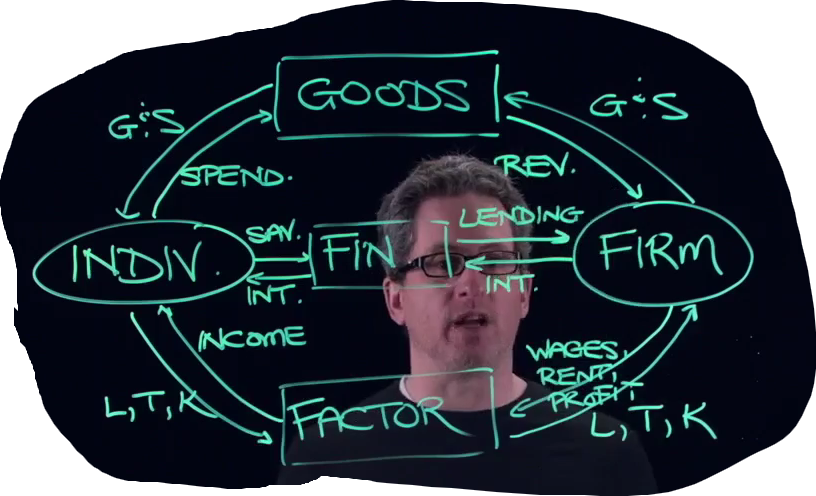
\includegraphics[width=0.5\textwidth]{CircularFlowOfIncomeAndExpenditure.png}
        \caption{Circular Flow of Income and Expenditure}
    \end{figure}
    Firms provide goods and services to the goods and services market and expect revenue.
    The factor market provides firms with resources (T, L and K) and expect wages, rent and profit.
    Individuals receive income (wages, rent and profit) from the factor market and provide resources (T, L and K).
    Individuals spend their income on goods and services in the goods and services market.
    Individuals save their income in the financial market and expect interest.
    Firms lend from the financial market and the market expects interest.

\end{example}

\subsection{}
Market Economy is generally the most efficient way to allocate resources. However, there are some limitations to the market economy.

Alternatives to the Market Economy:
\begin{itemize}
    \item Traditional Economy: Resources are allocated based on inheritance and custom. \begin{quote}"We've always done it that way."\end{quote}
    \item Command Economy: Resources are allocated by a centralized authority.
    \item Mixed Economy: Resources are allocated by a combination of market, tradition and command.
\end{itemize}

Gouvernment's Role in the Market Economy, correcting where the market fails:
\begin{itemize}
    \item Institutions
    \item Legal System
    \item Courts
    \item Justice
    \item Public Goods - Goods that cannot be efficiently provided by the market.
\end{itemize}

\section{Chapter 2}
\subsection{}

There are two ways to express economic statements:
\begin{itemize}
    \item \begin{definition}
        \emph{Positive statements} are factual statements. They do not always have to be factually correct.
        They just have to be presented as facts.
    \end{definition}
    \item \begin{definition}
        \emph{Normative statements} are value judgements or opinionated.
    \end{definition}
\end{itemize}
We do not need to worry about muddled statements that could be both positive and normative.
Neither positive nor normative statements are better than the other.
\begin{example}
    \begin{itemize}
        \item Positive: Today is Monday.\\
        Note: Whether or not today is Monday is not the point. The point is that it is presented as a factual statement.
        \item Normative: The minimum wage in Quebec is too low.
    \end{itemize}
\end{example}
\subsection{}

What's the process of presenting findings in \emph{Economic Analysis}?

Start with \emph{observations}.
As the world changes, our observations change with it.
We then develop \emph{theories} based on these observations.

\begin{example}
    We observe that every crisis leads to a rebound.
\end{example}

We then develop a theory into a \emph{model}. These models are mathematical.
Models are simplifications of reality.
The more realistic the model, the more accurate and the more complex it is.
Models have response, independent and dependent variables.

Within the model, there are some variables that are determined within the model itself, some are outside that we drop in and utilize.
An outside variable is called an \emph{exogenous or independent variable}. 
An inside variable is called an \emph{endogenous or dependent variable}, it is determined within the model. Given some parameters, we can this will determine a particular value of this variable in the model.
The more endogenous variables, the more complex the model.

In this course, you should be able to differentiate between exogenous, endogenous, indepedent and dependent variables.

Models are based on assumptions.
Recall that the Robinson Crusoe model was based on assumptions.

Why do economists disagree?\\
They disagree because they are making different assumptions which lead to different conclusions. To each party their assumptions are correct.
The role then is to make value judgements, ask: was this a positive or normative situation?

When drawing conclusions, be careful of what you are identifying:
\begin{itemize}
    \item \begin{definition} \emph{correlation} is a relationship between two variables but the relationship is not clear.\end{definition}
    \item \begin{definition} \emph{causation} is a relationship between two variables where one causes the other.\end{definition}
\end{itemize}
\begin{example}
    Women's skirts were worn higher when stock markets were up. This is a correlation. Both the stock market and skirt height were related to economic confidence. The stock market did not cause the skirt height to rise or vice versa.
\end{example}
\begin{example}
    Raising bank interest rates reduce consumer and business spending. This is causation. The bank interest rates caused the spending to decrease.
\end{example}
The causation or correlation relationship of some variables today may change tomorrow.
\end{document}